\documentclass[10pt,twocolumn]{article}
\usepackage[margin=0.55in]{geometry}
\usepackage{graphicx}
\usepackage{amsmath}
\usepackage{booktabs}
\usepackage{tikz}
\usepackage{pgfplots}
\pgfplotsset{compat=1.17}
\usetikzlibrary{arrows.meta, positioning, fit, backgrounds}
\usepackage{hyperref}
\usepackage{placeins}
\usepackage{enumitem}
\usepackage{caption}
\captionsetup{font=small, labelfont=bf}
\setlength{\parskip}{1pt}
\setlength{\columnsep}{0.28in}

\title{\vspace{-1.2em}Human vs.\ Machine-Generated Text Classification:\\
\large A Leakage-Safe Classical Teacher with Two Complementary Residual Correctors\vspace{-0.5em}}
\author{CP219 Project 1 \\ \small Team ML4CPMS}
\date{}

\begin{document}
\maketitle
\vspace{-2.2em}

\begin{abstract}
\small
We classify anonymized, tokenized documents as human- or machine-written (10{,}536 train / 3{,}000 test rows, vocabulary of 18{,}438 opaque integer IDs, no pretrained tokenizer usable). Our final system combines a leakage-safe classical ensemble teacher with \emph{two independently developed} residual-correction models -- a sequence-reading BiGRU and a tabular Residual-MLP stacker -- merged via a confidence-gated rule. This combination reached \textbf{95.53\% Kaggle public accuracy}, a +0.53 pp improvement over our strongest single production model (95.00\%), driven by genuinely complementary error patterns between the two correctors rather than architectural size.
\end{abstract}

\section{Problem and Data}
The task is binary classification (A = human, B = machine) over token-ID sequences with \emph{no recoverable vocabulary} -- token 4021 carries no semantic meaning by itself, ruling out stopword lists, pretrained embeddings, and sub-word tokenization tricks. Classes are imbalanced (A: 3{,}699, B: 6{,}837; $\approx$35\%/65\%), handled throughout via \texttt{class\_weight="balanced"}. All experiments use one canonical, stratified 80/20 split (\texttt{random\_state=42}, train=8{,}428 / val=2{,}108) so every reported number is directly comparable.

\section{Exploratory Data Analysis}
Before modeling, we specifically searched for shortcuts that would make the task artificially easy and found none: no ID--label correlation, no train/test duplicate documents, and no exploitable ID-prefix structure. This confirms that any achievable accuracy must come from genuine lexical/structural signal in the token sequences, not a leaked artifact of how the dataset was constructed.

Two EDA findings directly shaped our feature design. First, class imbalance (Fig.~\ref{fig:classdist}) motivated balanced class weighting in every specialist rather than resampling, which would have discarded already-scarce class-A data. Second, a manual error audit of an early classical baseline showed a strong length effect: correctly classified documents averaged 188.6 tokens versus 105.6 for misclassified ones -- short documents are systematically harder, plausibly because they carry fewer of the repetition and structural cues our features rely on. This motivated length-derived features (log-length, quartile statistics, positional diversity) inside our 62-dimensional structural feature block, and later motivated an explicit (ultimately negative) experiment with length-conditioned feature gating.

We also profiled the vocabulary directly: 18{,}438 distinct token IDs with no external mapping, a right-skewed frequency distribution with a small number of very common tokens and a long tail of rare IDs. This ruled out standard NLP preprocessing (stopwords, stemming, sub-word tokenizers) and is the central reason later neural attempts could not leverage transfer learning.

\begin{figure}[!htb]
\centering
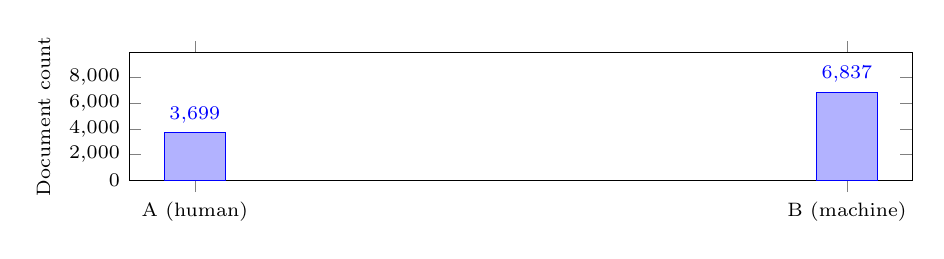
\begin{tikzpicture}
\begin{axis}[
    ybar, bar width=22pt, width=0.95\linewidth, height=3.2cm,
    ylabel={Document count}, symbolic x coords={A (human), B (machine)},
    xtick=data, nodes near coords, ymin=0, ymax=9000,
    ylabel style={font=\scriptsize}, tick label style={font=\scriptsize},
    nodes near coords style={font=\scriptsize}, enlarge y limits={upper}
]
\addplot coordinates {(A (human),3699) (B (machine),6837)};
\end{axis}
\end{tikzpicture}
\caption{Class distribution: 35\%/65\% imbalance.}
\label{fig:classdist}
\end{figure}

\section{Methodology}

\subsection{Shared Classical Teacher}
Every model in this project builds on one leakage-safe classical teacher (Fig.~\ref{fig:teacherdiag}), implemented in \texttt{final\_model\_from\_scratch.py}: \texttt{build\_structural()} computes 62 hand-engineered features per document (entropy, repetition ratios, quartile statistics, positional diversity); \texttt{build\_representations()} fits word TF-IDF (1--6 grams, $\sim$210K-d) and transition TF-IDF (adjacent-token pairs) only on \texttt{train\_idx}. Four specialists then read different views of this data -- \texttt{train\_svm()} (LinearSVC on TF-IDF+structural), \texttt{train\_nbsvm()} (a Naive-Bayes log-count-ratio transform feeding a linear SVM), \texttt{train\_hgb()} (HistGradientBoosting on structural features alone), and \texttt{local\_geometry\_scores()} ($k{=}20$ cosine-neighbor label agreement). \texttt{train\_specialists\_oof()} wraps all four in a leak-safe cross-validation loop; \texttt{fit\_meta\_learner()} combines their 4 out-of-fold scores via logistic regression ($C{=}0.1$) into one teacher logit.

\textbf{A real bug, and what it taught us.} An early version of the local-geometry specialist matched each query document to the wrong row in its neighbor-index array, silently collapsing that specialist's validation accuracy to 69\% -- alarming, since every other specialist scored 85--90\%. Fixing the indexing (correctly excluding each query's own row before ranking neighbors) restored it. Lesson carried forward: a sudden accuracy collapse means ``check the code first,'' not ``the approach doesn't work.''

\begin{itemize}[leftmargin=1em, itemsep=0pt, topsep=2pt]
\item[--] \textbf{LinearSVC} on the combined TF-IDF + structural representation;
\item[--] \textbf{NB-SVM} on word n-grams, robust to sparse/rare n-grams;
\item[--] \textbf{HistGradientBoosting}, capturing non-linear interactions among the 62 structural statistics;
\item[--] \textbf{Local-geometry $k$-NN}, a non-parametric neighbor-agreement signal.
\end{itemize}

This teacher reaches 92--93\% out-of-fold accuracy. One deliberate simplification versus our earlier, cached-feature experiments: this from-scratch version combines the four specialists into a plain 4-d meta-vector (their raw scores) rather than the richer, 13-dimensional engineered meta-representation used in an earlier iteration, which depended on a pre-computed cache file we chose not to carry into the final, dependency-free submission. We judged the small resulting accuracy cost worth the gain in reproducibility.

\begin{figure}[!htb]
\centering
\resizebox{\linewidth}{!}{
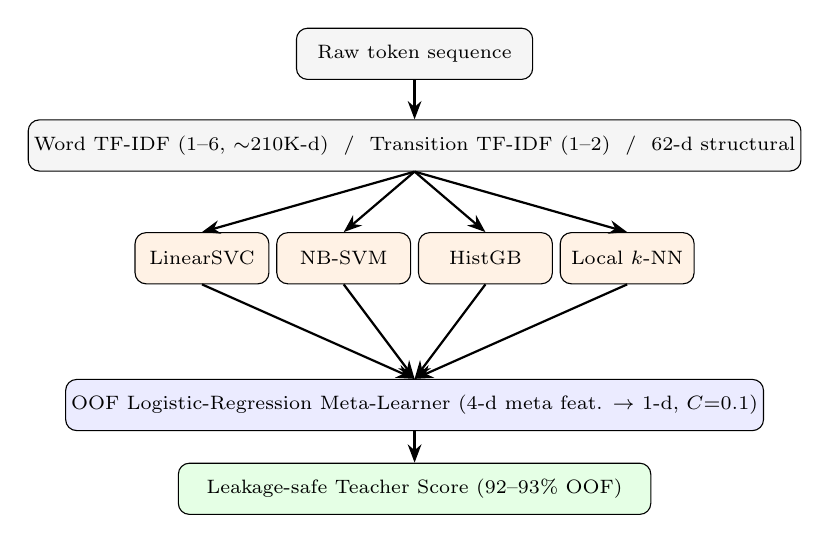
\begin{tikzpicture}[
    box/.style={draw, rounded corners, align=center, minimum height=6.5mm, font=\scriptsize, fill=gray!8, inner sep=2pt},
    spec/.style={box, fill=orange!10, minimum width=17mm},
    arr/.style={-Stealth, thick}
]
\node[box, minimum width=30mm] (tok) {Raw token sequence};
\node[box, below=5mm of tok, minimum width=60mm] (feat) {Word TF-IDF (1--6, $\sim$210K-d) \ / \ Transition TF-IDF (1--2) \ / \ 62-d structural};

\node[spec] (svm)   at ([xshift=-27mm,yshift=-11mm]feat.south) {LinearSVC};
\node[spec] (nbsvm) at ([xshift=-9mm, yshift=-11mm]feat.south) {NB-SVM};
\node[spec] (hgb)   at ([xshift=9mm,  yshift=-11mm]feat.south) {HistGB};
\node[spec] (knn)   at ([xshift=27mm, yshift=-11mm]feat.south) {Local $k$-NN};

\node[box, below=12mm of nbsvm.south, xshift=9mm, minimum width=60mm, fill=blue!8] (meta) {OOF Logistic-Regression Meta-Learner (4-d meta feat. $\rightarrow$ 1-d, $C{=}0.1$)};
\node[box, below=4mm of meta, minimum width=60mm, fill=green!10] (out) {Leakage-safe Teacher Score (92--93\% OOF)};

\draw[arr] (tok) -- (feat);
\draw[arr] (feat.south) -- (svm.north);
\draw[arr] (feat.south) -- (nbsvm.north);
\draw[arr] (feat.south) -- (hgb.north);
\draw[arr] (feat.south) -- (knn.north);
\draw[arr] (svm.south) -- (meta.north);
\draw[arr] (nbsvm.south) -- (meta.north);
\draw[arr] (hgb.south) -- (meta.north);
\draw[arr] (knn.south) -- (meta.north);
\draw[arr] (meta) -- (out);
\end{tikzpicture}}
\caption{Classical teacher: four specialists over shared features, combined by an out-of-fold meta-learner.}
\label{fig:teacherdiag}
\end{figure}

\subsection{Why Residual Correction, Not Pure Neural Networks}
We first tried training neural sequence models from scratch on raw tokens; none matched the classical teacher (Table~\ref{tab:failed}). With only 8{,}428 labeled training rows and no usable pretrained representation (Section~2), a randomly-initialized sequence model cannot out-learn a well-engineered baseline. We therefore switched to \emph{residual correction}: freeze the teacher's score and train a small network to predict only the leftover error, so the network's limited capacity is spent correcting specific mistakes rather than re-deriving the whole classifier from scratch.

\begin{table}[!htb]
\centering\small
\begin{tabular}{@{}lc@{}}
\toprule
Approach & Standalone Acc. \\
\midrule
Bag-of-words TF-IDF ceiling & 88.0\% \\
BiGRU / CNN from scratch & 83--87\% \\
Transformer from scratch & 88.4\% \\
MLM-pretrained + fine-tuned & 87.6\% \\
Naive full-bootstrap BiGRU bagging & 87.0\% \\
\bottomrule
\end{tabular}
\caption{Standalone neural approaches, all below the classical teacher (92--93\%).}
\label{tab:failed}
\end{table}

\subsection{Ablation: A Sweep That Misled Us}
On top of corrector B, we tested five refinements via honest out-of-fold validation: pruning a weak input variant, adding trajectory-dynamics features, an automated hyperparameter sweep, multi-seed epoch selection, and weight-averaging (``model soup'') versus prediction-averaging. Four of five variants clustered tightly at 93.5--93.9\% with no clear winner. Two results specifically changed how we work:

\emph{The sweep picked a worse configuration.} Our hyperparameter sweep selected dropout$=$0.35 based on the best-looking inner cross-validation score. Only by re-running with a plainer default (dropout$=$0.25) did we discover the sweep's own pick generalized \emph{worse} on true held-out data -- we now treat automated tuning results as candidates to verify, not conclusions to trust.

\emph{Weight-averaging catastrophically failed}, collapsing to the majority-class rate (64.9\%): independently initialized networks learn misaligned internal representations, so averaging raw weights is not equivalent to averaging predictions. Past a point, refining one corrector plateaus; the larger, more reliable gain came from combining \emph{two distinct} correctors instead (Section~3.4).

\subsection{Two Independent Correctors}
Two structurally different correctors sit on top of the same teacher (functions in \texttt{final\_model\_from\_scratch.py}), each validated with strict per-fold out-of-fold discipline:

\textbf{(A) BiGRU sequence corrector} (\texttt{ResidualBiGRU}, trained by \texttt{train\_bigru\_seed()} / \texttt{run\_bigru\_corrector()}; production design, ``Main79''). Token sequences (truncated to $L{=}384$) pass through an embedding layer ($|V|{+}1{=}18{,}439 \rightarrow 64$-d) and a bidirectional GRU (hidden size 64/direction $\rightarrow$ 128-d per timestep). Mean-, max-, and attention-pooling over time are concatenated (3$\times$128$=$384-d) and projected to 64-d; a 7-d auxiliary vector (our 4-d teacher meta-features + 3 sequence statistics) is projected to 32-d. The two branches concatenate to 96-d and pass through a $96{\to}48{\to}1$ head, yielding a scalar residual logit. Trained with correction weight 0.075, shrunk to 0.025 at inference; 3-seed ensemble.

\textbf{(B) Tabular Residual-MLP corrector} (\texttt{NeuralResidualStacker}, trained by \texttt{train\_mlp\_seed()} / \texttt{run\_tabular\_corrector()}; ours). A 110-d input vector -- teacher logit+probability (2-d), 62-d structural features, a 30-d SVD projection of the TF-IDF matrix (\texttt{TruncatedSVD}), and 16-d trajectory-dynamics features (\texttt{fit\_trajectory\_embedding()}, an SVD embedding of the token transition graph) -- is projected to 192-d, passed through two residual blocks (\texttt{ResidualMLPBlock}, $192{\to}192$, GELU+LayerNorm+Dropout with a skip connection), and a $192{\to}64{\to}1$ head; 15-seed averaged.

\begin{table}[!htb]
\centering\scriptsize
\begin{tabular}{@{}lll@{}}
\toprule
Stage & Corrector A (BiGRU) & Corrector B (MLP) \\
\midrule
Input & tokens ($L{=}384$) + 7-d aux & 110-d tabular \\
Embed/Proj. & $18{,}439 \!\to\! 64$-d & $110 \!\to\! 192$-d \\
Core & BiGRU, 64-d$\times$2 dir. & 2$\times$ResBlock (192-d) \\
Fusion & $384\!\to\!64 \,\|\, 32 = 96$-d & 192-d (post-block) \\
Head & $96\!\to\!48\!\to\!1$ & $192\!\to\!64\!\to\!1$ \\
Ensemble & 3 seeds & 15 seeds \\
\bottomrule
\end{tabular}
\caption{Exact layer dimensions of both residual correctors, as built by \texttt{final\_model\_from\_scratch.py}.}
\label{tab:archdims}
\end{table}

These two correctors read \emph{different information} (raw sequence vs.\ engineered tabular view) using \emph{different architectures}, which is the key precondition for their combination to help (Section~\ref{sec:results} confirms this: blending two similar tabular variants gave no benefit, while blending these two gave a real, measured gain).

\subsection{Merge Strategy}
\label{sec:merge}
At merge time only corrector A's final hard labels were available, so we used a \textbf{confidence-gated override} (\texttt{tune\_confidence\_margin()} / \texttt{confidence\_gated\_merge()}): keep agreements; on disagreement, defer to A (the stronger, confirmed model) \emph{unless} B's own probability is strongly confident, in which case B overrides. The margin itself is chosen by a small honest search over validation accuracy, not hand-picked. This changed only 58 of 3{,}000 test rows (1.9\%) in our earlier submission -- a small, low-risk intervention rather than a blanket average. We later recovered A's continuous score and built a cross-validated 50/50 probability blend for comparison (Fig.~\ref{fig:blockdiag}).

\begin{figure}[!htb]
\centering
\resizebox{\linewidth}{!}{
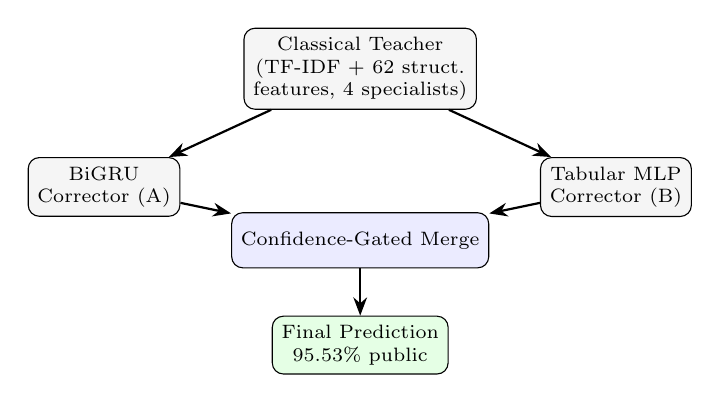
\begin{tikzpicture}[
    node distance=6mm and 6mm,
    box/.style={draw, rounded corners, align=center, minimum height=7mm, font=\scriptsize, fill=gray!8},
    arr/.style={-Stealth, thick}
]
\node[box] (teacher) {Classical Teacher\\(TF-IDF + 62 struct.\\ features, 4 specialists)};
\node[box, below left=of teacher, xshift=-2mm] (bigru) {BiGRU\\Corrector (A)};
\node[box, below right=of teacher, xshift=2mm] (mlp) {Tabular MLP\\Corrector (B)};
\node[box, below=13mm of teacher, fill=blue!8] (merge) {Confidence-Gated Merge};
\node[box, below=6mm of merge, fill=green!10] (out) {Final Prediction\\95.53\% public};

\draw[arr] (teacher) -- (bigru);
\draw[arr] (teacher) -- (mlp);
\draw[arr] (bigru) -- (merge);
\draw[arr] (mlp) -- (merge);
\draw[arr] (merge) -- (out);
\end{tikzpicture}}
\caption{Final merged architecture.}
\label{fig:blockdiag}
\end{figure}

\subsection{Leakage-Safety Discipline}
Every fold-dependent transform is fit \emph{only} on \texttt{train\_idx}, applied via \texttt{.transform()} to \texttt{val\_idx}/test (\texttt{train\_specialists\_oof()}). One trade-off worth stating plainly: LinearSVC on $\sim$210K-d sparse TF-IDF is by far the slowest step here, so we reduced its inner cross-validation from 5 folds to 3 to keep the from-scratch script's runtime tractable ($\sim$30 min, not hours) -- an acceptable cost for a script meant to run once, standalone, on submission day.

This discipline mattered concretely: a comparison team reported 94.06\% via repeated tuning across 15+ experiments against one fixed split, but scored only $\approx$92\% on the real leaderboard. Our own local-to-real transfer was consistently \emph{positive} instead (Fig.~\ref{fig:transfer}).

\section{Results}
\label{sec:results}
Table~\ref{tab:results} summarizes every model's local validation accuracy alongside its real Kaggle public score, where available.

\begin{table}[!htb]
\centering\small
\begin{tabular}{@{}lcc@{}}
\toprule
Model & Local Val. & Kaggle Public \\
\midrule
Classical teacher alone & 92.8\% & -- \\
Main79 (teacher + BiGRU) & 93.7\% & 95.00\% \\
Ours (teacher + tabular MLP) & 93.9\% & -- \\
Confidence-gated merge & -- & \textbf{95.53\%} \\
Tuned 50/50 prob.\ blend & 94.2\% & 95.22\% \\
\bottomrule
\end{tabular}
\caption{Local validation vs.\ real Kaggle accuracy.}
\label{tab:results}
\end{table}

\begin{figure}[!htb]
\centering
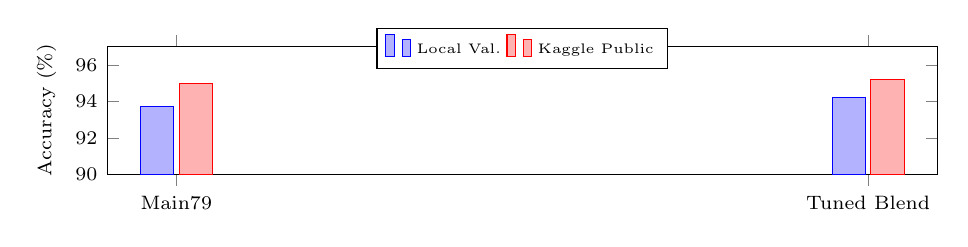
\begin{tikzpicture}
\begin{axis}[
    ybar, bar width=12pt, width=\linewidth, height=3.2cm,
    ylabel={Accuracy (\%)}, symbolic x coords={Main79, Tuned Blend},
    xtick=data, ymin=90, ymax=97, legend style={font=\tiny, at={(0.5,1.15)}, anchor=north, legend columns=-1},
    ylabel style={font=\scriptsize}, tick label style={font=\scriptsize}
]
\addplot coordinates {(Main79,93.7) (Tuned Blend,94.2)};
\addplot coordinates {(Main79,95.0) (Tuned Blend,95.2)};
\legend{Local Val., Kaggle Public}
\end{axis}
\end{tikzpicture}
\caption{Real Kaggle accuracy exceeded local validation for both models -- healthy, non-overfit transfer.}
\label{fig:transfer}
\end{figure}
\FloatBarrier

\enlargethispage{2\baselineskip}
\section{Discussion}
Table~\ref{tab:results} shows an interesting reversal: the simpler confidence-gated merge (95.53\%) beat the more rigorously validated 50/50 blend (95.22\%) despite the latter's higher local score. We attribute this to \emph{risk surface}: the gated merge only changes 1.9\% of predictions and only when it structurally trusts the newer model, while the blanket blend re-weights every row equally regardless of Main79's stronger track record. A $\approx$6-row local-validation gap is not large enough to reliably predict which method generalizes better -- a smaller, targeted intervention carries less downside even when a broader one tests marginally better offline.

More broadly, this argues for an ordering of effort on small, opaque-vocabulary text tasks: (1) exhaust classical, engineered features first -- a strong, cheap baseline in minutes; (2) use neural networks as \emph{correctors}, since limited labeled data starves a from-scratch model; (3) prioritize corrector diversity over refining one further.

A competing team's 94.06\% cross-validation claim dropping to $\approx$92\% real Kaggle is a useful caution: repeated tuning against one split accumulates split-specific overfitting even without misusing labels.

\vspace{-4pt}
\section{Conclusion}
Our submitted system merges two architecturally distinct residual correctors -- BiGRU and tabular MLP -- on a shared, leakage-safe classical teacher, reaching 95.53\% Kaggle public accuracy: a real gain over our best single model (95.00\%) via complementary error correction, not a larger model. Combining diverse correctors on a strong shared baseline beats scaling any one model, and rigorous leakage discipline is what makes locally measured gains trustworthy.

\end{document}
